\subsection{Build, Deployment and release via CI/CD pipeline in AWS[ Md Yousuf Ali Khan]}\label{sec:build-task-aws}
We used the AWS ECS (Amazon Elastic Container Service) service to deploy our application, a fully managed container orchestration service that enables us to deploy, manage, and scale containerized applications. We created a new docker image for every new release of our application and uploaded that docker image into Amazon ECR (Elastic Container Registry), which is a private container registry. AWS ECS uses that container image, takes care of the scaling of our application, and manages our containers for availability. By using AWS ECS, we will not have to worry about the scalability of our application. In figure~\ref{sec:build-task-aws} the build job for creating a build for the newly modified code in the repository is presented.

\begin{figure}[h]
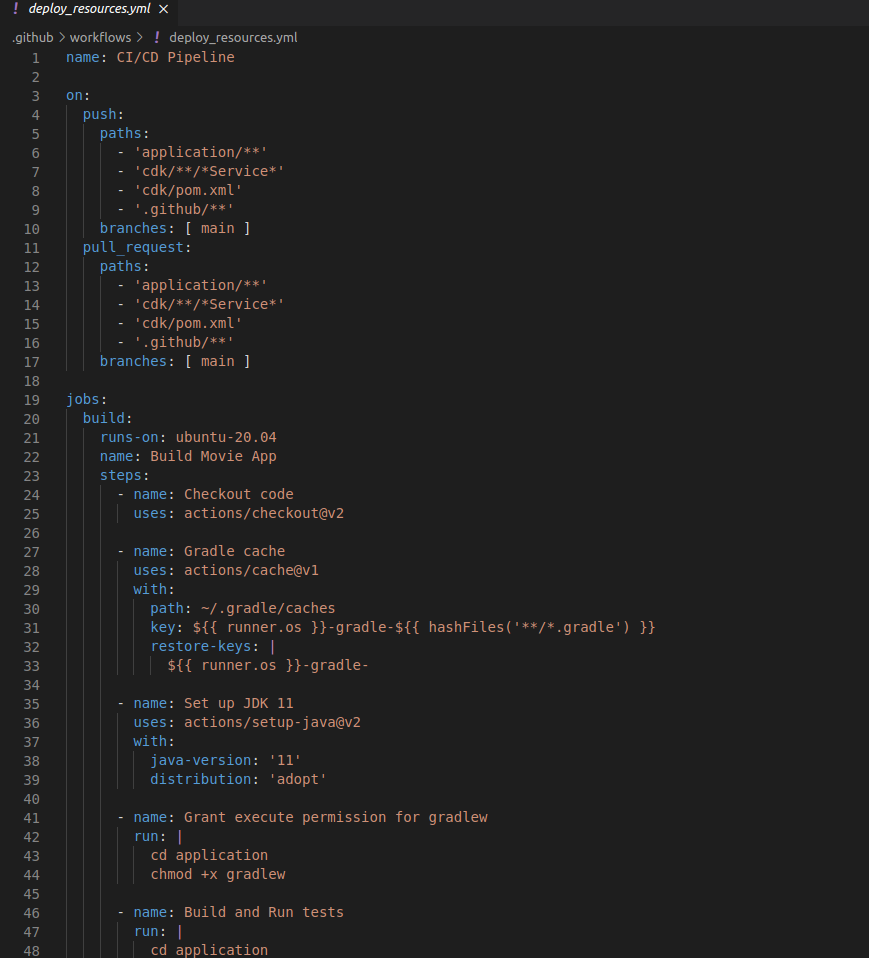
\includegraphics[scale=0.40]{images/yousuf/build-job-aws-github.png}
\centering
\caption{The {{CI\CD}} pipeline build task in Github workflow file}
\label{fig:ci-cd-build-task}
\end{figure}




